\documentclass[9pt]{beamer}

% Beamer style
%\usetheme[secheader]{Madrid}
% \usetheme{CambridgeUS}
\useoutertheme{infolines}
\usecolortheme[rgb={0.65,0.15,0.25}]{structure}
% \usefonttheme[onlymath]{serif}
\beamertemplatenavigationsymbolsempty
%\AtBeginSubsection

% Packages
%\usepackage[french]{babel}
\usepackage[latin1]{inputenc}
\usepackage{color}
% \usepackage[dvipsnames]{xcolor}
\usepackage{xspace}
\usepackage{dsfont, stmaryrd}
\usepackage{amsmath, amsfonts, amssymb, stmaryrd, mathabx}
\usepackage{epsfig}
\usepackage{multirow}
\usepackage{tikz}
\usepackage{url}
% \usepackage{ulem}
\usepackage{/home/robin/LATEX/Biblio/astats}
%\usepackage[all]{xy}
\usepackage{graphicx}

% Maths
% \newtheorem{theorem}{Theorem}
% \newtheorem{definition}{Definition}
\newtheorem{proposition}{Proposition}
% \newtheorem{assumption}{Assumption}
% \newtheorem{algorithm}{Algorithm}
% \newtheorem{lemma}{Lemma}
% \newtheorem{remark}{Remark}
% \newtheorem{exercise}{Exercise}
% \newcommand{\propname}{Prop.}
% \newcommand{\proof}{\noindent{\sl Proof:}\quad}
% \newcommand{\eproof}{$\blacksquare$}

% \setcounter{secnumdepth}{3}
% \setcounter{tocdepth}{3}
\newcommand{\pref}[1]{\ref{#1} p.\pageref{#1}}
\newcommand{\qref}[1]{\eqref{#1} p.\pageref{#1}}

% Colors : http://latexcolor.com/
\definecolor{darkred}{rgb}{0.65,0.15,0.25}
\definecolor{darkgreen}{rgb}{0,0.4,0}
\definecolor{darkred}{rgb}{0.65,0.15,0.25}
\definecolor{amethyst}{rgb}{0.6, 0.4, 0.8}
\definecolor{asparagus}{rgb}{0.53, 0.66, 0.42}
\definecolor{applegreen}{rgb}{0.55, 0.71, 0.0}
\definecolor{awesome}{rgb}{1.0, 0.13, 0.32}
\definecolor{blue-green}{rgb}{0.0, 0.87, 0.87}
\definecolor{red-ggplot}{rgb}{0.52, 0.25, 0.23}
\definecolor{green-ggplot}{rgb}{0.42, 0.58, 0.00}
\definecolor{purple-ggplot}{rgb}{0.34, 0.21, 0.44}
\definecolor{blue-ggplot}{rgb}{0.00, 0.49, 0.51}

% Commands
\newcommand{\backupbegin}{
   \newcounter{finalframe}
   \setcounter{finalframe}{\value{framenumber}}
}
\newcommand{\backupend}{
   \setcounter{framenumber}{\value{finalframe}}
}
\newcommand{\emphase}[1]{\textcolor{darkred}{#1}}
\newcommand{\comment}[1]{\textcolor{gray}{#1}}
\newcommand{\paragraph}[1]{\textcolor{darkred}{#1}}
\newcommand{\refer}[1]{{\small{\textcolor{gray}{{\cite{#1}}}}}}
\newcommand{\Refer}[1]{{\small{\textcolor{gray}{{[#1]}}}}}
\newcommand{\goto}[1]{{\small{\textcolor{blue}{[\#\ref{#1}]}}}}
\renewcommand{\newblock}{}

\newcommand{\tabequation}[1]{{\medskip \centerline{#1} \medskip}}
% \renewcommand{\binom}[2]{{\left(\begin{array}{c} #1 \\ #2 \end{array}\right)}}

% Variables 
\newcommand{\Abf}{{\bf A}}
\newcommand{\Beta}{\text{B}}
\newcommand{\Bcal}{\mathcal{B}}
\newcommand{\Bias}{\xspace\mathbb B}
\newcommand{\Cor}{{\mathbb C}\text{or}}
\newcommand{\Cov}{{\mathbb C}\text{ov}}
\newcommand{\cl}{\text{\it c}\ell}
\newcommand{\Ccal}{\mathcal{C}}
\newcommand{\cst}{\text{cst}}
\newcommand{\Dcal}{\mathcal{D}}
\newcommand{\Ecal}{\mathcal{E}}
\newcommand{\Esp}{\xspace\mathbb E}
\newcommand{\Espt}{\widetilde{\Esp}}
\newcommand{\Covt}{\widetilde{\Cov}}
\newcommand{\Ibb}{\mathbb I}
\newcommand{\Fcal}{\mathcal{F}}
\newcommand{\Gcal}{\mathcal{G}}
\newcommand{\Gam}{\mathcal{G}\text{am}}
\newcommand{\Hcal}{\mathcal{H}}
\newcommand{\Jcal}{\mathcal{J}}
\newcommand{\Lcal}{\mathcal{L}}
\newcommand{\Mt}{\widetilde{M}}
\newcommand{\mt}{\widetilde{m}}
\newcommand{\Nbb}{\mathbb{N}}
\newcommand{\Mcal}{\mathcal{M}}
\newcommand{\Ncal}{\mathcal{N}}
\newcommand{\Ocal}{\mathcal{O}}
\newcommand{\pt}{\widetilde{p}}
\newcommand{\Pt}{\widetilde{P}}
\newcommand{\Pbb}{\mathbb{P}}
\newcommand{\Pcal}{\mathcal{P}}
\newcommand{\Qcal}{\mathcal{Q}}
\newcommand{\qt}{\widetilde{q}}
\newcommand{\Rbb}{\mathbb{R}}
\newcommand{\Sbb}{\mathbb{S}}
\newcommand{\Scal}{\mathcal{S}}
\newcommand{\st}{\widetilde{s}}
\newcommand{\St}{\widetilde{S}}
\newcommand{\Tcal}{\mathcal{T}}
\newcommand{\todo}{\textcolor{red}{TO DO}}
\newcommand{\Ucal}{\mathcal{U}}
\newcommand{\Un}{\math{1}}
\newcommand{\Vcal}{\mathcal{V}}
\newcommand{\Var}{\mathbb V}
\newcommand{\Vart}{\widetilde{\Var}}
\newcommand{\Zcal}{\mathcal{Z}}

% Symboles & notations
\newcommand\independent{\protect\mathpalette{\protect\independenT}{\perp}}\def\independenT#1#2{\mathrel{\rlap{$#1#2$}\mkern2mu{#1#2}}} 
\renewcommand{\d}{\text{\xspace d}}
\newcommand{\gv}{\mid}
\newcommand{\ggv}{\, \| \, }
% \newcommand{\diag}{\text{diag}}
\newcommand{\card}[1]{\text{card}\left(#1\right)}
\newcommand{\trace}[1]{\text{tr}\left(#1\right)}
\newcommand{\matr}[1]{\boldsymbol{#1}}
\newcommand{\matrbf}[1]{\mathbf{#1}}
\newcommand{\vect}[1]{\matr{#1}} %% un peu inutile
\newcommand{\vectbf}[1]{\matrbf{#1}} %% un peu inutile
\newcommand{\trans}{\intercal}
\newcommand{\transpose}[1]{\matr{#1}^\trans}
\newcommand{\crossprod}[2]{\transpose{#1} \matr{#2}}
\newcommand{\tcrossprod}[2]{\matr{#1} \transpose{#2}}
\newcommand{\matprod}[2]{\matr{#1} \matr{#2}}
\DeclareMathOperator*{\argmin}{arg\,min}
\DeclareMathOperator*{\argmax}{arg\,max}
\DeclareMathOperator{\sign}{sign}
\DeclareMathOperator{\tr}{tr}
\newcommand{\ra}{\emphase{$\rightarrow$} \xspace}

% Hadamard, Kronecker and vec operators
\DeclareMathOperator{\Diag}{Diag} % matrix diagonal
\DeclareMathOperator{\diag}{diag} % vector diagonal
\DeclareMathOperator{\mtov}{vec} % matrix to vector
\newcommand{\kro}{\otimes} % Kronecker product
\newcommand{\had}{\odot}   % Hadamard product

% TikZ
\newcommand{\nodesize}{2em}
\newcommand{\edgeunit}{2.5*\nodesize}
\newcommand{\edgewidth}{1pt}
\tikzstyle{node}=[draw, circle, fill=black, minimum width=.75\nodesize, inner sep=0]
\tikzstyle{square}=[rectangle, draw]
\tikzstyle{param}=[draw, rectangle, fill=gray!50, minimum width=\nodesize, minimum height=\nodesize, inner sep=0]
\tikzstyle{hidden}=[draw, circle, fill=gray!50, minimum width=\nodesize, inner sep=0]
\tikzstyle{hiddenred}=[draw, circle, color=red, fill=gray!50, minimum width=\nodesize, inner sep=0]
\tikzstyle{observed}=[draw, circle, minimum width=\nodesize, inner sep=0]
\tikzstyle{observedred}=[draw, circle, minimum width=\nodesize, color=red, inner sep=0]
\tikzstyle{eliminated}=[draw, circle, minimum width=\nodesize, color=gray!50, inner sep=0]
\tikzstyle{empty}=[draw, circle, minimum width=\nodesize, color=white, inner sep=0]
\tikzstyle{blank}=[color=white]
\tikzstyle{nocircle}=[minimum width=\nodesize, inner sep=0]

\tikzstyle{edge}=[-, line width=\edgewidth]
\tikzstyle{edgebendleft}=[-, >=latex, line width=\edgewidth, bend left]
\tikzstyle{edgebendright}=[-, >=latex, line width=\edgewidth, bend right]
\tikzstyle{lightedge}=[-, line width=\edgewidth, color=gray!50]
\tikzstyle{lightedgebendleft}=[-, >=latex, line width=\edgewidth, bend left, color=gray!50]
\tikzstyle{lightedgebendright}=[-, >=latex, line width=\edgewidth, bend right, color=gray!50]
\tikzstyle{edgered}=[-, line width=\edgewidth, color=red]
\tikzstyle{edgebendleftred}=[-, >=latex, line width=\edgewidth, bend left, color=red]
\tikzstyle{edgebendrightred}=[-, >=latex, line width=\edgewidth, bend right, color=red]

\tikzstyle{arrow}=[->, >=latex, line width=\edgewidth]
\tikzstyle{arrowbendleft}=[->, >=latex, line width=\edgewidth, bend left]
\tikzstyle{arrowbendright}=[->, >=latex, line width=\edgewidth, bend right]
\tikzstyle{arrowred}=[->, >=latex, line width=\edgewidth, color=red]
\tikzstyle{arrowbendleftred}=[->, >=latex, line width=\edgewidth, bend left, color=red]
\tikzstyle{arrowbendrightred}=[->, >=latex, line width=\edgewidth, bend right, color=red]
\tikzstyle{arrowblue}=[->, >=latex, line width=\edgewidth, color=blue]
\tikzstyle{dashedarrow}=[->, >=latex, dashed, line width=\edgewidth]
\tikzstyle{dashededge}=[-, >=latex, dashed, line width=\edgewidth]
\tikzstyle{dashededgebendleft}=[-, >=latex, dashed, line width=\edgewidth, bend left]
\tikzstyle{lightarrow}=[->, >=latex, line width=\edgewidth, color=gray!50]


% Directory
\newcommand{\figcp}{/home/robin/RECHERCHE/RUPTURES/EXPOSES/FIGURES}
\newcommand{\figeco}{/home/robin/RECHERCHE/ECOLOGIE/EXPOSES/FIGURES}
\newcommand{\fignet}{/home/robin/RECHERCHE/RESEAUX/EXPOSES/FIGURES}
\newcommand{\figbayes}{/home/robin/RECHERCHE/BAYES/EXPOSES/FIGURES}
% \newcommand{\figDLR}{/home/robin/Bureau/Hawkes/segHP/article/StatComp2023/Revision/figures}
\newcommand{\figchiro}{/home/robin/RECHERCHE/RUPTURES/Hawkes/HawkesDiscreteHMM/Figures/chiropteres}
\newcommand{\figsimul}{/home/robin/RECHERCHE/RUPTURES/Hawkes/HawkesDiscreteHMM/Figures/simuls}
\newcommand{\figStR}{/home/robin/RECHERCHE/BAYES/PLNsampling/Paper/Figures}

%====================================================================
%====================================================================

%====================================================================
%====================================================================
\begin{document}
%====================================================================
%====================================================================

%====================================================================
\title{Some latent variable models in ecology}

\author[S. Robin]{St�phane Robin \\ ~ \\
    Joint works with Anna Bonnet, Julien Chiquet, Pierre Latouche, \\
    Mahendra Mariadassou, Sarah Ouadah, Julien Stoehr
}

\institute[Sorbonne universit�]{\normalsize{LPSM, Sorbonne universit�}}

\date[StatMathAppli'25]{StatMathAppli, Fr�jus, Sep. 2025}

%====================================================================
%====================================================================
\maketitle

%====================================================================
\section*{Introduction}
%====================================================================
%====================================================================
\subsection*{Latent variable models}
%====================================================================
\frame{\frametitle{Latent variable models (1/2)} 

  \paragraph{Latent  ('hidden', 'unobserved', ...) variables} are widely used in statistical ecology  \refer{PeG22b} to 
  \begin{itemize}
    \setlength{\itemsep}{.75\baselineskip}
    \item account for heterogeneity (species clustering, over-dispersion or 'excess' of counts), 
    \item encode dependency (due to space, time, parental relatedness, ...), 
    \item represent a 'true' signal, observed with noise (animal movement and/or behavior), 
    \item ...
  \end{itemize}

  \bigskip \bigskip \pause
  \paragraph{Statistical perspective.} 
  \begin{itemize}
    \setlength{\itemsep}{.75\baselineskip}
    \item Number of latent variables $\simeq$ number of observed variables.
    \item Inference of the model parameters much easier if the latent variables were observed.
  \end{itemize}
}

%====================================================================
\frame{\frametitle{Latent variable models (2/2)} 

\paragraph{Notations.}
  \begin{itemize}
    \item $Y =$ observed variables of interest (response),
    \item $Z =$ unobserved (latent) variables,
    \item $\theta =$ unknown parameter (to be inferred),
    \item $X =$ covariates,
  \end{itemize}

  \bigskip \bigskip \pause 
  \paragraph{General model.}
  \begin{align*}
      \text{hidden layer:} \qquad \qquad Z & \sim p_\theta(Z; \textcolor{gray}{X}), \\ ~ \\
      \text{observed layer:} \qquad Y \mid Z & \sim p_\theta(Y \mid Z; \textcolor{gray}{X}).
  \end{align*}

}

%====================================================================
\frame{\frametitle{Graphical model} 

  \begin{tabular}{cc}
    \hspace{-.04\textwidth}
    \begin{tabular}{p{.5\textwidth}}
      \begin{itemize}
        \item $Y =$ response,
        \item $Z =$ latent,
        \item $\theta =$ parameter,
        \item $X =$ covariates
      \end{itemize}
    \end{tabular}
    & 
    \hspace{-.25\textwidth}
    \begin{tabular}{p{.5\textwidth}}
      \input{\figeco/GMlatentVarModel-XYZtheta}
    \end{tabular}
  \end{tabular}
  
  \bigskip \bigskip \pause
  \paragraph{Nature of the variables.}
  $$
  \begin{tabular}{l|cc}
    & Fixed & Random \\
    \hline
    & \\
    Observed & covariates $\emphase{X}$ & response $\emphase{Y}$ \\
    & \\
    Unobserved & parameter $\emphase{\theta}$ & latent $\emphase{Z}$
  \end{tabular}
  $$
}

%====================================================================
\frame{\frametitle{Inference specificity} 

  \paragraph{'Observed likelihood'} = likelihood of the observed data $Y$:
  $$
  p_\theta(Y) 
  = 
  \int_\Zcal p_\theta(Z) p_\theta(Y \mid Z) \d Z
  $$
  \pause
  but (EM decomposition \refer{DLR77})
  $$
  \log p_\theta(Y) = \Esp[\log p_\theta(Y, Z) \mid Y] + \Hcal(p_\theta(Z \mid Y)
  $$
  where $\Hcal$ stands for the entropy\footnote{$\Hcal(q) = - \Esp_q[\log q(X)]$}.
  
  \bigskip \bigskip \pause
  \paragraph{Three typical situations:}
  \begin{enumerate}
    \setlength{\itemsep}{.75\baselineskip}
    \item \pause Integration wrt $Z$ can be done for free,
    \item \pause Integration wrt $Z$ is intractable, but $p_\theta(Z \mid Y)$ is accessible,
    \item \pause Integration wrt $Z$ is intractable, and $p_\theta(Z \mid Y)$ is inaccessible.
  \end{enumerate}

}

\setcounter{tocdepth}{1}
\frame{\frametitle{Outline} \tableofcontents}

%====================================================================
\section{Motifs in plant-pollinator networks}
\setcounter{tocdepth}{2}
\frame{\frametitle{Outline} \tableofcontents[currentsection]}
%====================================================================
%====================================================================
\subsection*{Bipartite expected degree distribution}
\frame{\frametitle{Bipartite expected degree distribution} 
}
%====================================================================

%====================================================================
%====================================================================
\subsection{Motif count distribution}
\frame{\frametitle{Motif count distribution under BEDD} 
}
%====================================================================

%====================================================================
%====================================================================
\subsection{Comparing networks in space and time}
\frame{\frametitle{Arsenic experimental design} 
}
%====================================================================



%====================================================================
\section{Markov switching Hawkes process \& Animal behavior}
\frame{\frametitle{Outline} \tableofcontents[currentsection]}
%====================================================================
%====================================================================
\subsection{A hidden Markov model?} 
\frame{\frametitle{Discrete time Markov-switching Hawkes process} 
%====================================================================

  \bigskip 
  \paragraph{Data.} $Y_k =$ number of bat calls during the $k$-th time bin.

  \bigskip \pause
  \paragraph{Markov switching Hawkes process model.} In discrete time:
  \begin{itemize}
    \setlength{\itemsep}{.75\baselineskip}
    \item Hidden path $(Z_k)_{k \geq 1} =$ homogeneous Markov chain with $Q$ states
    $$
    (Z_k)_{k \geq 1} \sim MC_Q(\nu, \pi)
    $$
    $\nu =$ intial distribution, $\pi =$ transition matrix;
    \item Observed counts: for $k\geq 1$ and
      $$
      \left(Y_k \mid (Y_\ell)_{\ell \leq k-1}, \emphase{Z_k=q}\right) 
      \sim \mathcal{P}\left(\emphase{\mu_q} + \alpha \sum_{\ell = 1}^{k-1} \beta^{\ell-1}Y_{k-\ell} \right);
      $$  
    \item Model parameters: $\theta = (\nu, \pi, \mu, \alpha, \beta)$
  \end{itemize}
  
  \bigskip \pause
  \paragraph{Proposition: Identifiability \refer{BoR25}\footnote{The proof does not rely on \refer{AMR09}}.}
  \begin{itemize}
    \setlength{\itemsep}{.75\baselineskip}
    \item The model parameter $\theta$ is identifiable from the joint distribution $p_\theta(Y_1, Y_2, Y_3)$. \\
    \textcolor{gray}{($\theta \neq \theta' \Rightarrow p_\theta(\cdot, \cdot, \cdot) \neq p_{\theta'}(\cdot, \cdot, \cdot)$)} 
  \end{itemize}

}

%====================================================================
\frame{\frametitle{Markovian representation (homogeneous case)} 

  \paragraph{Homogeneous discrete-time Hawkes process $Y = \{Y_k\}_{k \geq 1}$.} 
  $$
  Y_k \mid (Y_\ell)_{\ell \leq k-1} \sim \mathcal{P}\left(\mu + \alpha \sum_{\ell = 1}^{k-1}\beta^{\ell-1} Y_{k-\ell} \right)
  $$
  \bigskip
  $(Y_k)_{k\geq 1}$ is not a Markov chain (because of infinite memory).

  \bigskip \pause
  \paragraph{Markovian representation.}
  \begin{itemize}
    \item Define
    $$
    U_1 = 0, \qquad \qquad 
    U_k = \alpha \sum_{\ell = 1}^k \beta^{\ell-1} Y_{k-\ell}, 
    $$
    \item \pause then, for $k \geq 1$ \textcolor{gray}{(with $U_0 = Y_0 = 0$)}
    $$
    U_k = {\alpha Y_{k-1} + \beta U_{k-1}}, 
    \qquad \qquad 
    Y_k \mid U_k \sim \mathcal{P}(\mu + U_k).
    $$
  \end{itemize}
  \pause 
  \medskip
  so $\left((Y_k,U_k)\right)_{k \geq 1}$ forms a Markov chain.
  
}

%====================================================================
\frame{\frametitle{Markovian representation (Markov switching case)} 

  \paragraph{Markov switching Hawkes process model.} Can be rephrased as
  $$
  \left(Y_k \mid (Y_\ell)_{\ell \leq k-1}, \emphase{Z_k=q}\right) 
  \sim \mathcal{P}\left(\emphase{\mu_q} + U_k \right)
  $$  
  with
  $$
  U_1 = 0, \qquad \qquad 
  U_k = \alpha \sum_{\ell = 1}^k \beta^{\ell-1} Y_{k-\ell}, 
  $$      
  
  \bigskip \pause
  \paragraph{Consequence.}
  \begin{itemize}
    \setlength{\itemsep}{.75\baselineskip}
    \item The model is a regular Hidden Markov Model (HMM)
    \item With graphical model
    \begin{figure}
      \begin{centering}
        \begin{tikzpicture}
\node[] (Zt_2) at (-\edgeunit, \edgeunit) {}; 
\node[] (Zt_1) at (0, \edgeunit) {$Z_{k-1}$}; 
\node[] (Zt) at (\edgeunit, \edgeunit) {$Z_{k}$}; 
\node[] (Zt1) at (2*\edgeunit, \edgeunit) {$Z_{k+1}$}; 
\node[] (Zt2) at (3*\edgeunit, \edgeunit) {}; 
\node[] (Ut_1) at (-0.5*\edgeunit, 0.5*\edgeunit) {$U_{k-1}$}; 
\node[] (Ut) at (0.5*\edgeunit, 0.5*\edgeunit) {$U_{k}$}; 
\node[] (Ut1) at (1.5*\edgeunit, 0.5*\edgeunit) {$U_{k+1}$}; 
\node[] (Ut2) at (2.5*\edgeunit, 0.5*\edgeunit) {$U_{k+2}$}; 
\node[] (Ut3) at (3.5*\edgeunit, 0.5*\edgeunit) {}; 
\node[] (Yt_2) at (-\edgeunit, 0) {}; 
\node[] (Yt_1) at (0, 0) {$Y_{k-1}$}; 
\node[] (Yt) at (\edgeunit, 0) {$Y_{k}$}; 
\node[] (Yt1) at (2*\edgeunit, 0) {$Y_{k+1}$}; 
\node[] (Yt2) at (3*\edgeunit, 0) {}; 

\draw[->,dashed] (Zt_2) -- (Zt_1); \draw[->] (Zt_1) -- (Zt); \draw[->] (Zt) -- (Zt1); \draw[->,dashed] (Zt1) -- (Zt2);
\draw[->] (Zt_1) -- (Yt_1); \draw[->] (Zt) -- (Yt); \draw[->] (Zt1) -- (Yt1);
\draw[->] (Ut_1) -- (Yt_1); \draw[->] (Ut) -- (Yt); \draw[->] (Ut1) -- (Yt1);
\draw[->] (Ut_1) -- (Ut); \draw[->] (Ut) -- (Ut1); \draw[->] (Ut1) -- (Ut2); \draw[->,dashed] (Ut2) -- (Ut3);
\draw[->,dashed] (Yt_2) -- (Ut_1); \draw[->] (Yt_1) -- (Ut); \draw[->] (Yt) -- (Ut1); \draw[->] (Yt1) -- (Ut2);
\end{tikzpicture}
 \\
        $(Z_k)_{k \geq 1} =$ \emphase{hidden path}, 
        $\quad (U_k)_{k \geq 1} =$ memory, 
        $\quad (Y_k)_{k \geq 1} =$ observed process.
      \end{centering}
    \end{figure}
  \end{itemize}
}

%====================================================================
\frame{\frametitle{Inference}

  \bigskip
  \paragraph{Maximum likelihood inference:} 
  $
  \widehat{\theta} = \argmax_\theta \log p_\theta(Y)
  $

  \bigskip \bigskip \pause
  \paragraph{EM algorithm for HMM:} \refer{DLR77,CMR05}
  $$
  \theta^{(h+1)} 
  = \underset{\text{\normalsize \emphase{M step}}}{\underbrace{\argmax_\theta}} \; \underset{\text{\normalsize \emphase{E step}}}{\underbrace{\Esp_{\theta^{(h)}}}}[\log p_\theta(Y, Z) \mid Y]
  $$
  \begin{itemize}
    \setlength{\itemsep}{.75\baselineskip}
    \item E step: Evaluate $Q(\theta \mid \theta^{(h)}) = \Esp_{\theta^{(h)}}[\log p_\theta(Y, Z) \mid Y]$ (forward-backward recursion)
    \item M step: Gradient descent, computing $\nabla_\theta Q(\theta \mid \theta^{(h)})$ by recursion
  \end{itemize}

  \bigskip \bigskip \pause
  \paragraph{Model selection.} Penalized likelihood
  \begin{align*}
    AIC_Q & = \log p_{\widehat{\theta}_Q}(Y) - D_Q, &
    BIC_Q & = \log p_{\widehat{\theta}_Q}(Y) - D_Q \frac{\log(\emphase{N})}2     
  \end{align*}
  with $D_Q =$ number of parameters $= 2 + Q^2$ and \emphase{$N =$ number of time bins}.
}

%====================================================================
\frame{ \frametitle{Simulation study (not shown)}
  
  \paragraph{Design.}
  \begin{itemize}
    \setlength{\itemsep}{.75\baselineskip}
    \item Simulate a \emphase{continuous time} Markov-switching Hawkes process
    \item With more or less events (control parameter $\lambda$)
    \item Then \emphase{discretise} with more or less bins (control parameter $N \; \propto$ nb events)
  \end{itemize}

  \bigskip \pause
  \paragraph{Conclusions.}
  \begin{itemize}
    \setlength{\itemsep}{.75\baselineskip}
    \item Inference more accurate when more signal (large $\lambda$)!!!
    \goto{back:HawkesFit}
    \item Inference more accurate with thinner discretization step (large $N$) \\
    But at the price of a higher computational cost  \goto{back:HawkesClassif}
    \item BIC does not capture the right number of states \\
    \textcolor{gray}{Sequences not simulated according to the model}
    \item AIC does, with reasonable signal ($\lambda$) and discretization ($N$) \\
    \textcolor{gray}{Blind to the simulation shift from the model?} \goto{back:HawkesAIC}
%     \item Clear advantage wrt Poisson HMM.
  \end{itemize} \label{sec:HawkesSimuls}
  
  \bigskip \pause
  \paragraph{Practical recommendations:}
  Take $N = 2 n$ \quad and \quad use AIC to choose $Q$.

}
    
%====================================================================
%====================================================================
\subsection{Bats calls sequences}
\frame{\frametitle{Bats calls sequences}} 
%====================================================================

%====================================================================
\frame{\frametitle{Vigie-chiro project} 

  \bigskip
  \paragraph{Data set.}
  \begin{itemize}
    \item Vigie-chiro project French participatory project to monitor bats echolocation calls (\url{https://www.vigienature.fr/fr/chauves-souris}).
    \item 2354 overnight recordings collected between October 2010 and January 2020 in 755 locations. 
    \item Restricted to sequences with at least 50 cries $\to$ 1555 time sequences. 
  \end{itemize}
  
  \bigskip \bigskip \pause
  \paragraph{Poisson vs Hawkes / Homogeneous vs HMM.} Best model according to AIC
  $$
  \begin{tabular}{r|cc|c}
    & Poisson & Hawkes & Total \\
    \hline
    Homogeneous & 34 & 353 & 387\\
    Hidden Markov  & 24 & \emphase{1144} & \emphase{1168} \\
    \hline
    Total & 58 & \emphase{1497} & 1555
  \end{tabular}
  $$
  \begin{itemize}
    \item Memory ($95\%$) and heterogeneity ($75\%$) are present in most sequences 
    \item Hawkes-HMM best fits almost 3 sequences out of 4.
  \end{itemize}

}

%====================================================================
\frame{ \frametitle{An example}

  $$
  \begin{tabular}{ccc}
    Hawkes HMM ($\widehat{Q} = 3$) & \qquad &
    Poisson HMM ($\widehat{Q} = 4$) \\ 
    ~ \\
    \includegraphics[width=.3\textwidth, trim=10 40 20 50, clip=]{\figchiro/Chiro-seq1776-N1048-Qmax5-classif-seg} &
    \qquad & 
    \includegraphics[width=.3\textwidth, trim=10 40 20 50, clip=]{\figchiro/Chiro-seq1776-N1048-Qmax5-classifP-seg} 
  \end{tabular}
  $$
  \bigskip
  \begin{itemize}
    \setlength{\itemsep}{.75\baselineskip}
    \item Interpretation of the states: \textcolor{red}{absence} of calls, transit and \textcolor{green}{foraging} (high call frequency)
    \item Hawkes-HMM state changes do not correspond to slope changes
    \item Poisson-HMM needs many state changes to account for self-excitation
  \end{itemize}
}
    
%====================================================================
\frame{ \frametitle{States and species}

  The number of bat species was also recorded each night
  
  $$
  \includegraphics[width=.45\textwidth]{\figchiro/boxplot_species_Coef2_allQ.pdf}
  $$
  \begin{itemize}
    \setlength{\itemsep}{.75\baselineskip}
    \item The number of states does not match the number of species
    \item More discussion to come with members of the Vigie-chiro project
  \end{itemize}

}


%====================================================================
\section{Joint species distribution model}
\frame{\frametitle{Outline} \tableofcontents[currentsection]}
%====================================================================
%====================================================================
\subsection{(Joint) species distribution models}
%====================================================================
\frame{\frametitle{(Joint) species distribution models} 

  \paragraph{Aim.} 
  Describe/understand the relationships that living species share with each other and with their environment (biogeography, community ecology). 

  \bigskip \bigskip \pause 
  \paragraph{Species distribution models.} 
  $n$ sites, $x_i =$ vector of environmental descriptors for site $i$, $Y_i =$ number of individual from the species of interest observed in site $i$:
  $$
  Y_i \sim \Fcal(\cdot; x_i, \emphase{\beta}).
  $$
  $\to$ Generalized linear (mixed) model \refer{ElL09,ZIW09}

  \bigskip \bigskip \pause
  \paragraph{Joint species distribution models.} 
  Same, but $Y_i = (Y_{i1}, \dots Y_{ip}) =$ vector of counts for $p$ species of interest observed in site $i$:
  $$
  Y_i \sim \Fcal_p(\cdot; x_i, \emphase{\beta}, \emphase{\Sigma})
  $$
  $\to$ Multivariate generalized linear mixed model  \refer{WBO15,OvA20}
  
}

%====================================================================
\frame{\frametitle{Poisson log-normal model}

  \bigskip
  \paragraph{A joint species distribution model:} 
  Poisson-log normal distribution \refer{AiH89,CMR21}
  \begin{align*}
    & \text{in each site $i = 1 \dots n$:} & 
    \emphase{Z_i} & \sim \Ncal_p(0, \emphase{\Sigma}) \\
    & \text{for each specie $j = 1 \dots p$:} &
    Y_{ij} \mid Z_{ij} & \sim \Pcal(\exp(x_i^\top \emphase{\beta_j} + Z_{ij}))
  \end{align*} \pause
  \begin{itemize}
    \setlength{\itemsep}{.5\baselineskip}
    \item $\emphase{\beta_j} =$ effects of the environmental covariates on species $j$ (\emphase{\sl abiotic} interactions)
    \item $\emphase{\Sigma} =$ between-species \textcolor{gray}{latent} covariance matrix  (\emphase{\sl biotic} interactions)
  \end{itemize}

  \bigskip \bigskip \pause
  \paragraph{Fish species from the Barents sea.} 
  $n = 89$ sites, $p = 30$ species, $d = 4$ covariates
  $$
  \begin{tabular}{ccc}
    Covariate effects & 
    Correlation induced & 
    Between species \\
    $\widehat{B}$ & 
    by the environment & 
    correlation  $\widehat{\Sigma}$ \\
    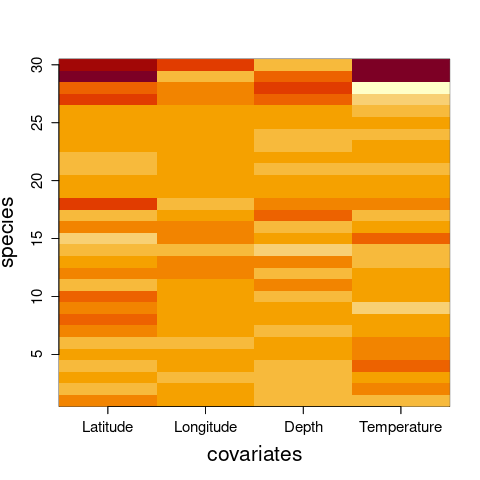
\includegraphics[width=.25\textwidth, trim=0 10 20 10, clip=]{\figbayes/FigUVSQ-BarentsFish-coeffAll-woIntercept-specOrderTRUE} & 
    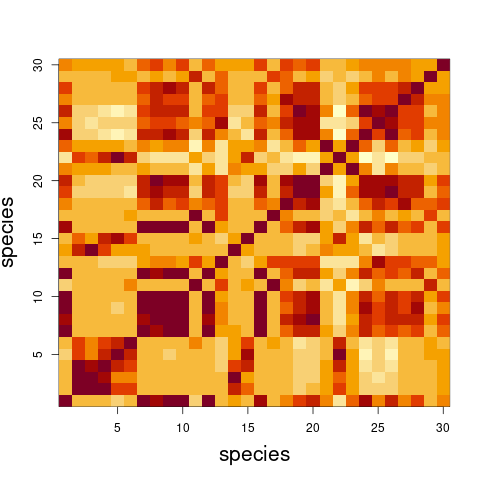
\includegraphics[width=.25\textwidth, trim=0 10 20 10, clip=]{\figbayes/FigUVSQ-BarentsFish-corrPred-specOrderTRUE} & 
    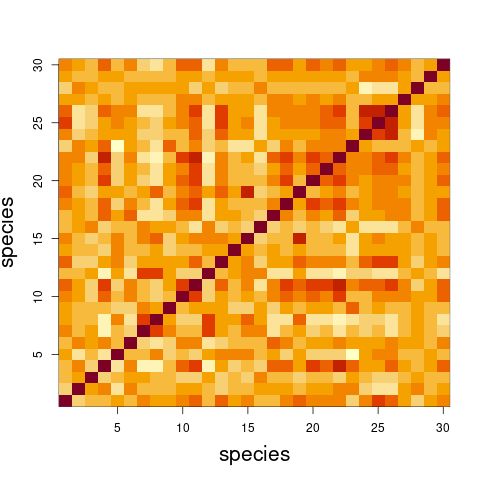
\includegraphics[width=.25\textwidth, trim=0 10 20 10, clip=]{\figbayes/FigUVSQ-BarentsFish-corrAll-specOrderTRUE}
  \end{tabular}
  $$
}

%====================================================================
%====================================================================
\subsection{From EM to Variational EM}
% \frame{\frametitle{Outline} \tableofcontents[currentsubsection]}
%====================================================================
\frame{\frametitle{Maximum likelihood with latent variables}

  \paragraph{Latent variable model.} Three ingredients:
  \begin{enumerate}
    \item $\emphase{\theta} =$ set of parameters:
    \begin{align*}
      \text{PLN:} \quad \theta & = (B, \Sigma) &
      \text{SBM:} \quad \theta & = (\pi, \alpha, \beta)
    \end{align*}
    \item $\emphase{Z} =$ set of latent variables:
    \begin{align*}
      Z & \sim p_\theta(Z) &
      (\text{PLN:\; multivariate normal, SBM:\; multinomial})
    \end{align*}
    \item $\emphase{Y} =$ set of observed variables:
    \begin{align*}
      Y & \sim p_\theta(Y \mid Z) &
      (\text{PLN \& SBM:\; Poisson})
    \end{align*}
  \end{enumerate}

  \bigskip \bigskip \pause
  \paragraph{Maximum likelihood inference.} Estimate $\theta$ with
  $$
  \widehat{\theta}
  = \argmax_\theta \; \log p_\theta(Y) 
  = \argmax_\theta \; \log \underset{\text{\normalsize Most often intractable}}{\underbrace{\int p_\theta(Y \mid z) p_\theta(z) \d z}} 
  $$

}

%====================================================================
\frame{\frametitle{EM algorithm}

  \paragraph{Expectation-Maximisation algorithm \refer{DLR77}.} $\theta^{(h)} =$ current value of the estimate,
  \begin{itemize}
    \item \emphase{E} step: Evaluate
    $$
    Q(\theta \mid \theta^{(h)}) := \Esp_{\theta^{(h)}}\left[\emphase{\log p_\theta(Y, Z)} \mid Y\right]
    $$
    \item \emphase{M} step: Update
    $$
    \theta^{(h+1)} = \argmax_\theta Q(\theta \mid \theta^{(h)})
    $$
  \end{itemize}
  $\to$ The log-likelihood increases at each step: $\log p_{\theta^{(h+1)}}(Y) \geq \log p_{\theta^{(h)}}(Y)$ .
  
  \bigskip \bigskip \pause
  \paragraph{Critical step = E step:} Requires to determine the conditional distribution
  $$
  p_\theta(Z \mid Y),
  $$
  or at least some of its moments.

  
  \bigskip \bigskip \pause
  \paragraph{Problem.} 
  For many models (including PLN and SBM), the E step is intractable 
}

%====================================================================
\frame{\frametitle{Variational EM (VEM) algorithm}

  \bigskip
  \paragraph{Principle \refer{WaJ08,BKM17}.} Replace the E step with an approximation step, i.e. \\ ~
  \begin{itemize}
    \setlength{\itemsep}{1\baselineskip}
    \item \pause Choose a class $\Qcal$ of approximate (parametric) distributions
    \item \pause Choose divergence measure $D[q \| p]$ (e.g. $KL[q \| p]$)
    \item \pause \emphase{VE} step : (approximation)
    $$
    q^{(h+1)} = \argmin_{q \in \emphase{\Qcal}} \emphase{D}\left[q(Z) \| p_{\theta^{(h)}}(Z \mid Y)\right]
    $$
    \item \pause \emphase{M} step : (update)
    $$
    \theta^{(h+1)} = \argmax_\theta \Esp_{\emphase{q^{(h+1)}}}\left[\log p_\theta(Y, Z)\right]
    $$
  \end{itemize}
  \pause
  \bigskip
  $\to$ If $D = KL$, a lower bound of $\log p_\theta(Y)$ ('ELBO') increases at each step
}
  
%====================================================================
\frame{\frametitle{Variational estimates}

  \bigskip 
  \textcolor{gray}{\paragraph{Remark:} A Bayesian version of it exists (Variational Bayes EM = VBEM).}

  \bigskip \bigskip \pause
  \paragraph{Pros:} Reasonably easy to implement, fast, empirically accurate
  
  \bigskip \bigskip \pause
  \paragraph{Cons:} Few theoretical guaranties \refer{CDP12,BCC13,MaM15}, does not enjoy the general properties of maximum likelihood (consistency, asymptotic normality, etc.) \\
  \medskip 
  $\to$ No measure of uncertainty (\emphase{no test, no confidence interval}) 
  
  \bigskip \bigskip \pause
  \paragraph{Question:} 
  Can we build upon variational inference to achieve 'genuine' statistical inference?

}

%====================================================================
%====================================================================
\subsection{Species abundances: Poisson log-normal model}
% \frame{\frametitle{Outline} \tableofcontents[currentsubsection]}
%====================================================================
\frame{\frametitle{Example 1: Variational EM (VEM) for the Poisson log-normal model}

  \paragraph{Model.} 
  $n$ sites, $p$ species
  \begin{align*}
    & \text{in each site $i = 1 \dots n$:} & 
    \emphase{Z_i} & \sim \Ncal_p(0, \emphase{\Sigma}) &
    & (\text{latent vector}) \\
    & \text{for each species $j = 1 \dots p$:} &
    Y_{ij} \mid Z_{ij} & \sim \Pcal(\exp(x_i^\top \emphase{\beta_j} + Z_{ij})) &
    & (\text{observed abundances})
  \end{align*} 
  
  \bigskip \pause
  \paragraph{No EM.} 
  The $Z_i$'s are marginally Gaussian, but not Gaussian conditionally on the $Y_{ij}$'s \\
  (no close form for $p(Z \mid Y)$, even in one dimension)
  
  \bigskip \bigskip \pause
  \paragraph{Variational EM.} Gaussian approximation \refer{CMR18a}
  $$
  q(Z) = \prod_{i=1}^n \Ncal(Z_i; m_i, S_i)
  $$
  \begin{itemize}
  \item Parameter estimate $\widehat{\theta} = (\widehat{\Sigma}, \widehat{\beta})$, 
  \item Approximate conditional distribution $Z_i \mid Y_i \approx \Ncal(\widetilde{m}_i, \widetilde{S}_i)$, 
  \item Lower bound $ELBO(\widehat{\theta}, \widetilde{m}, \widetilde{S})$ (R package \url{PLNmodels})
  \end{itemize}
  
}

%====================================================================
\frame{\frametitle{Toward genuine maximum likelihood inference \refer{StR24}}

  \pause
  \paragraph{Monte Carlo EM.} \refer{CeD85} When $p(Z \mid Y)$ intractable:
  \begin{itemize}
    \item Monte Carlo E step: Sample $(Z^m)_{m = 1 \dots M} \overset{iid}{\sim} p_{\theta^{(h)}}(Z \mid Y)$, then estimate
    $$
    \widehat{Q}(\theta \mid \theta^{(h)}) := \frac1{M} \sum_{m=1}^M \log p_\theta(Y, Z^m)
    $$
    \item M step: Update
    $$
    \theta^{(h+1)} = \argmax_\theta \widehat{Q}(\theta \mid \theta^{(h)}) 
    $$
  \end{itemize}

  \bigskip \bigskip \pause
  \paragraph{Importance sampling. }
  How to sample from $p_{\theta^{(h)}}(Z \mid Y)$?
  \begin{itemize}
   \item Sample $(Z^m)_{m = 1 \dots M} \overset{iid}{\sim} q^{(h)}(Z)$, $q^{(h)} =$ proposal,
   \item Compute the non-normalized weights $\rho_m^{(h)} = p_{\theta^{(h)}}(Y, Z^m) \left/ q^{(h)}(Z^m)\right.$,
   \item \pause Estimate
    $$
    \widehat{Q}(\theta \mid \theta^{(h)}) := \sum_{m=1}^M \rho_m^{(h)} \log p_\theta(Y, Z^m) \; \left/ \; \sum_{m=1}^M \rho_m^{(h)} \right.,
    $$
  \end{itemize}

}

%====================================================================
\frame{\frametitle{Composite likelihood}

  \bigskip
  \paragraph{Importance sampling has a poor efficiency\footnote{Measured in terms of ESS $\simeq$ variance of the weights}} in 'large' dimension (say $p \geq 10, 15$) \\
  \medskip 
  $\to$ Need to reduce the sampling dimension

  \bigskip \bigskip \pause
  \paragraph{Composite likelihood.} 
  \begin{itemize}
    \item Build $B$ overlapping blocks $\Ccal_1, \dots \Ccal_B$, each containing $k$ species, 
    \item Define the composite log-likelihood as
    $$
    \cl_\theta(Y) = \sum_{b=1}^B \log p_\theta(Y^b), 
    \qquad
    \text{where} \quad 
    Y^b = [Y_{ij}]_{i = 1, \dots n, j \in \Ccal_b},
    $$
    \item \pause Then, the maximum composite likelihood estimator \refer{VRF11}
    $$
    \widehat{\theta}_{CL} = \argmax_\theta \cl_\theta(Y) 
    $$
    is consistent, asymptotically Gaussian with asymptotic variance given by
    \begin{align*}
      J(\theta) & = \Var_\theta[\nabla_\theta \cl_\theta(Y)], 
      \qquad \qquad 
      H(\theta) = - \Esp_\theta[\nabla^2_\theta \cl_\theta(Y)], \\
      \Var_\infty(\widehat{\theta}_{CL}) & = H^{-1}(\theta) J(\theta) H^{-1}(\theta).
    \end{align*} 
  \end{itemize}

}

%====================================================================
\frame{\frametitle{Proposed composite likelihood algorithm}

  \paragraph{Dealing with latent variables.}
  \begin{itemize}
    \item The latent variables $Z$ can be split in the same way as the observed abundances $Y$:
    $$
    Z^b = [Z_{ij}]_{i = 1, \dots n, j \in \Ccal_b},
    $$
    \item The EM algorithm can be extended to composite log-likelihood \\
    \textcolor{gray}{(Proof: apply the EM decomposition within each block)}
  \end{itemize}

  \bigskip \bigskip \pause
  \paragraph{Proposal for importance sampling.}
  \begin{itemize}
    \item Start with $q_b^{(1)}(Z^b) = \qt_{VEM}(Z^b)$
    \item Then update $q_b^{(h+1)}(Z^b)$ with the estimated mean and variance of $p_{\theta^{(h)}}(Z^b \mid Y^b)$.
  \end{itemize}

  \bigskip \bigskip \pause
  \paragraph{Building the blocks.} To guaranty the same precision for all estimates, one would ideally want that
  \begin{itemize}
    \item[$\beta_j$:] Each species $j$ belongs to the same number of blocks $\Ccal_1, \dots \Ccal_B$
    \item[$\sigma_{jj'}$:] Each pair of species $(j, j')$ appears in the same number of blocks 
    \item Same problem as the construction of a incomplete balanced block design\footnote{Not always possible: need to have $p \mid Bk$ and $p(p-1) \mid Bk(k-1)$}
  \end{itemize}

}

%====================================================================
\frame{\frametitle{Simulation study}

  \paragraph{Main aim.} Assess normality 
  \begin{itemize}
    \item Test statistic $(\widehat{\theta} -\theta^*) \left/ \sqrt{\widehat{\Var}_\infty(\widehat{\theta})} \right.$ for the regression coefficients
    \item Criterion = $p$-value of the Kolmogorov-Smirnov test for normality
  \end{itemize}
  
  \bigskip \bigskip \pause
  \paragraph{Results.} $100$ sites, $3$ covariates, $100$ simulations
  \newcommand{\lagSim}{50} \newcommand{\nISsim}{200} \newcommand{\nIterSim}{1000}
  \newcommand{\simulParms}{-nIter\nIterSim-lag\lagSim-nIS\nISsim}
  $$
  \begin{tabular}{cccc}
    7 species & 10 species & 20 species & 50 species \\
    \includegraphics[width=.2\textwidth, trim=10 10 25 25, clip=]{\figStR/PvalKS-score-n100-d3-p7-parm1\simulParms} & 
    \includegraphics[width=.2\textwidth, trim=10 10 25 25, clip=]{\figStR/PvalKS-score-n100-d3-p10-parm1\simulParms} & 
    \includegraphics[width=.2\textwidth, trim=10 10 25 25, clip=]{\figStR/PvalKS-score-n100-d3-p20-parm1\simulParms} &
    \includegraphics[width=.2\textwidth, trim=10 10 25 25, clip=]{\figStR/PvalKS-score-n100-d3-p50-parm1\simulParms}  
  \end{tabular}
  $$
  FL = full likelihood, CL$k$ = composite likelihood$(k = \textcolor{gray}{2}, 3, \textcolor{gray}{5}, 7)$, \\
  \medskip
  \textcolor{gray}{VEM = pseudo Fisher information based on the ELBO},  \\
  JK = jackknife variance estimate of $\Var(\widehat{\theta}_{VEM})$

}

%====================================================================
\frame{\frametitle{Fish species in the Barents sea}

  \newcommand{\nIterEx}{10000} \newcommand{\lagEx}{50} \newcommand{\nISex}{200}
  \newcommand{\exampleParms}{-nIter\nIterEx-lag\lagEx-nIS\nISex}
  \newcommand{\nIterSel}{\nIterEx} \newcommand{\lagSel}{20} \newcommand{\nISsel}{\nISex}
  \newcommand{\selectParms}{-nIS\nISsel-nIter\nIterSel-lag\lagSel}
  
  \bigskip
  \paragraph{Comparison of the estimates.}
  $$
  \begin{tabular}{ccc}
    $\widehat{B}$ & $\widehat{\Sigma}$ & ESS (CL5) \\
    \includegraphics[width=.25\textwidth, trim=10 10 25 50, clip=]{\figStR/Barents\exampleParms-compBeta-cem5-all} & 
    \includegraphics[width=.25\textwidth, trim=10 10 25 50, clip=]{\figStR/Barents\exampleParms-compSigma-cem5-all} & 
    \includegraphics[width=.25\textwidth, trim=10 10 25 50, clip=]{\figStR/Barents\exampleParms-ESS-cem5}     
  \end{tabular}
  $$

  \pause
  \paragraph{Significance.} Test statistics $\widehat{\theta} \left/ \sqrt{\widehat{\Var}_\infty(\widehat{\theta})} \right.$
  $$
  \begin{tabular}{ccc}
    $\widehat{B}$ & $\widehat{\Sigma}$ & $\text{cor}(\widehat{\Sigma})$ \\
    \includegraphics[width=.25\textwidth, trim=10 10 25 25, clip=]{\figStR/Barents\exampleParms-betaSignif-cem5} & 
    \includegraphics[width=.25\textwidth, trim=10 10 25 25, clip=]{\figStR/Barents\exampleParms-sigmaSignif-cem5} &
    \includegraphics[width=.25\textwidth, trim=10 10 25 25, clip=]{\figStR/Barents\exampleParms-corSigmaSignif-cem5}
  \end{tabular}  
  $$
}




%====================================================================
\frame[allowframebreaks]{ \frametitle{References} \allowbreak
  {
   \tiny
   \bibliography{/home/robin/Biblio/BibGene}
   \bibliographystyle{alpha}
  }
}

%====================================================================
%====================================================================
\backupbegin 

%====================================================================
\section*{Network motifs}
%==================================================================
\frame{\frametitle{Bipartite motifs} \label{back:motifList}

  \label{sec:motifList}
  \begin{tabular}{ll}
    \hspace{-.04\textwidth}
    \begin{tabular}{p{.45\textwidth}}
      \paragraph{'Meso-scale' analysis.} \refer{SCB19}
      \begin{itemize}
       \item Motifs ='building-blocks'
       \item between local (several nodes) and global (sub-graph)
      \end{itemize}
      \bigskip \bigskip 
      \paragraph{Interest.}
      \begin{itemize}
       \item Generic description of a network
       \item Enables network comparison
       \item Even when the nodes are different
      \end{itemize} \\
      \textcolor{gray}{($+$ 'species-role': out of the scope here)} \\
      \goto{sec:motifs}
    \end{tabular}
    &
    \begin{tabular}{p{.45\textwidth}} 
      \hspace{-0.035\textwidth}
      \includegraphics[width=.45\textwidth]{\fignet/SCB19-Oikos-Fig3-6motifs} \\      
    \end{tabular} 
  \end{tabular}

  \bigskip \bigskip 
  \paragraph{Existing tool.} \url{bmotif} package \refer{SSS19}: counts motif occurrences (\emphase{Not an easy task!})

}

%==================================================================
\frame{\frametitle{\BEDD model} \label{back:BEDD}

  \begin{tabular}{cccc}
    & & $h_0(v) =$ & $h(v) =$ \\
    \multicolumn{2}{c}{
      $\begin{array}{rl}
        \Pbb\{i \sim j \mid U_i, V_j\} & = \rho \; g(U_i) \; h(V_j) \\ \\
        \Esp (Y_{i+} \mid U_i) & = n \; \rho \; g(U_i) \\ \\
        \Esp (Y_{+j} \mid V_j) & = m \; \rho \; g(V_i) 
      \end{array}$
    } &
    \begin{tabular}{c} 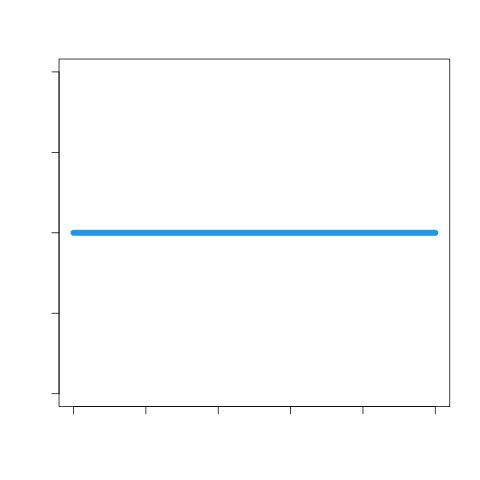
\includegraphics[width=.18\textwidth]{\fignet/FigMotifsBEDD-dist-h10} \end{tabular} &
    \begin{tabular}{c} 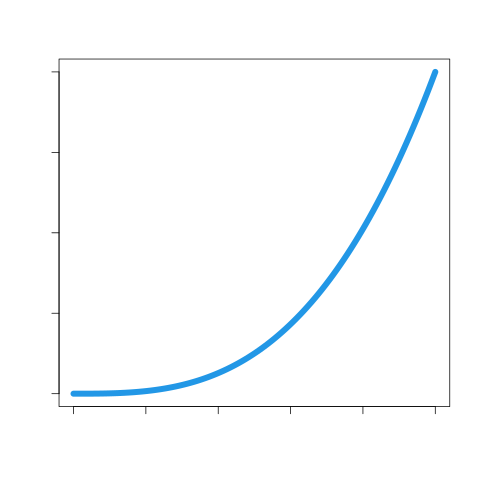
\includegraphics[width=.18\textwidth]{\fignet/FigMotifsBEDD-dist-h40} \end{tabular} \\
    \begin{tabular}{c} $g_0(u) =$ \end{tabular} &
    \begin{tabular}{c} 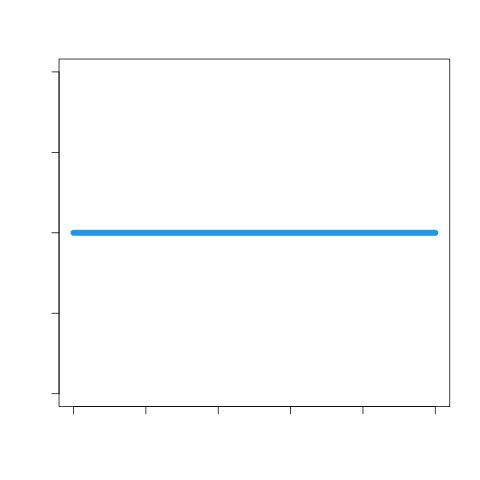
\includegraphics[width=.18\textwidth]{\fignet/FigMotifsBEDD-dist-g10} \end{tabular} &
    \begin{tabular}{c} 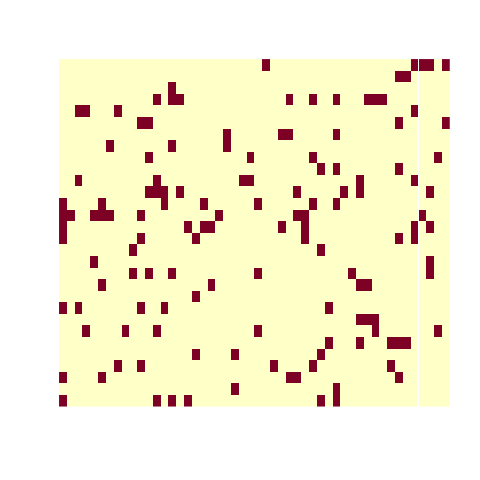
\includegraphics[width=.18\textwidth]{\fignet/FigMotifsBEDD-adj-g10-h10} \end{tabular} &
    \begin{tabular}{c} 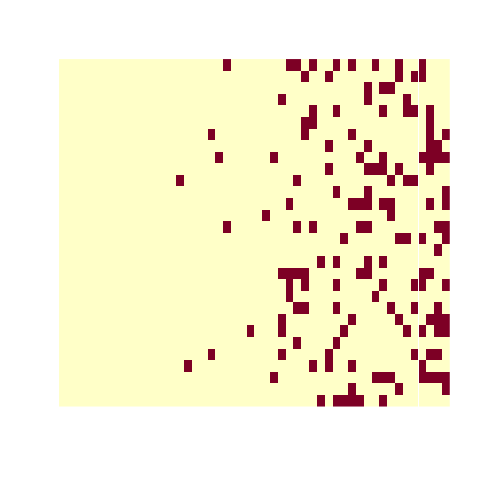
\includegraphics[width=.18\textwidth]{\fignet/FigMotifsBEDD-adj-g10-h40} \end{tabular} \\
    \begin{tabular}{c} $g(u) =$ \end{tabular} &
    \begin{tabular}{c} 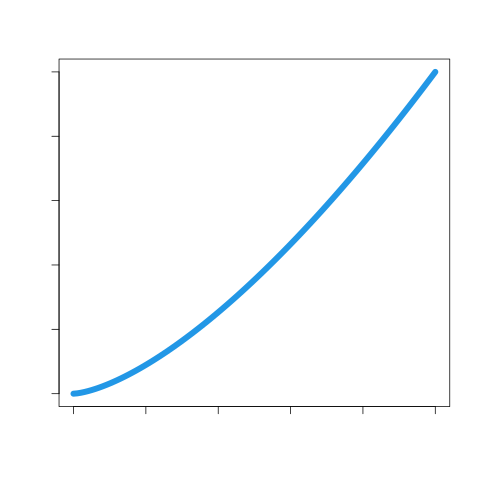
\includegraphics[width=.18\textwidth]{\fignet/FigMotifsBEDD-dist-g25} \end{tabular} &
    \begin{tabular}{c} 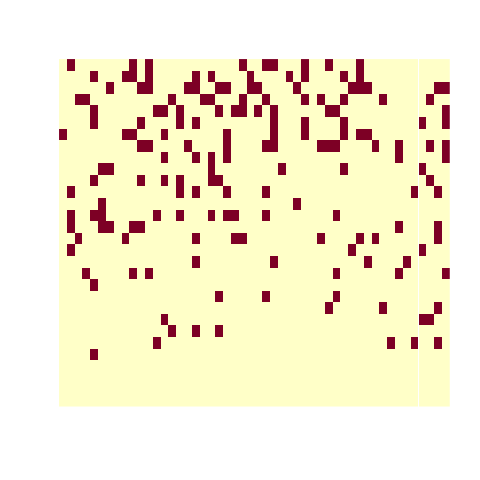
\includegraphics[width=.18\textwidth]{\fignet/FigMotifsBEDD-adj-g25-h10} \end{tabular} &
    \begin{tabular}{c} 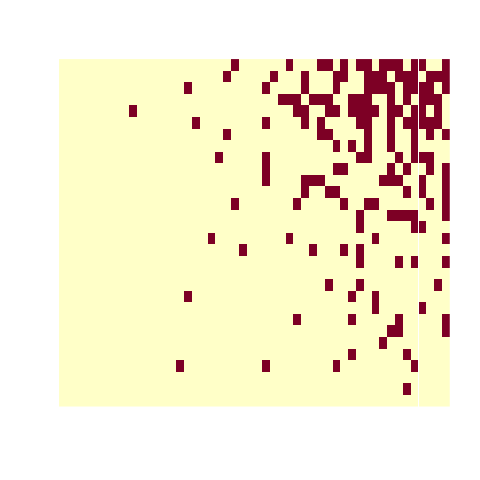
\includegraphics[width=.18\textwidth]{\fignet/FigMotifsBEDD-adj-g25-h40} \end{tabular} \\
  \end{tabular}
  
  \goto{sec:BEDD}
}



%====================================================================
\section*{Hawkes discrete HMM}
%====================================================================
\frame{\frametitle{Self-exciting exponential Hawkes process} \label{back:Hawkes}

  $$
  \lambda(t)= \lambda_0 + a \underset{T_k < t}{\sum} e^{-b(t-T_k)}
  $$
  \paragraph{Self exciting:} 
  Each event increases the probability of observing another event
  
  \bigskip \bigskip \pause
  \begin{tabular}{cc}
    \hspace{-.04\textwidth}
    \begin{tabular}{p{.4\textwidth}}
%       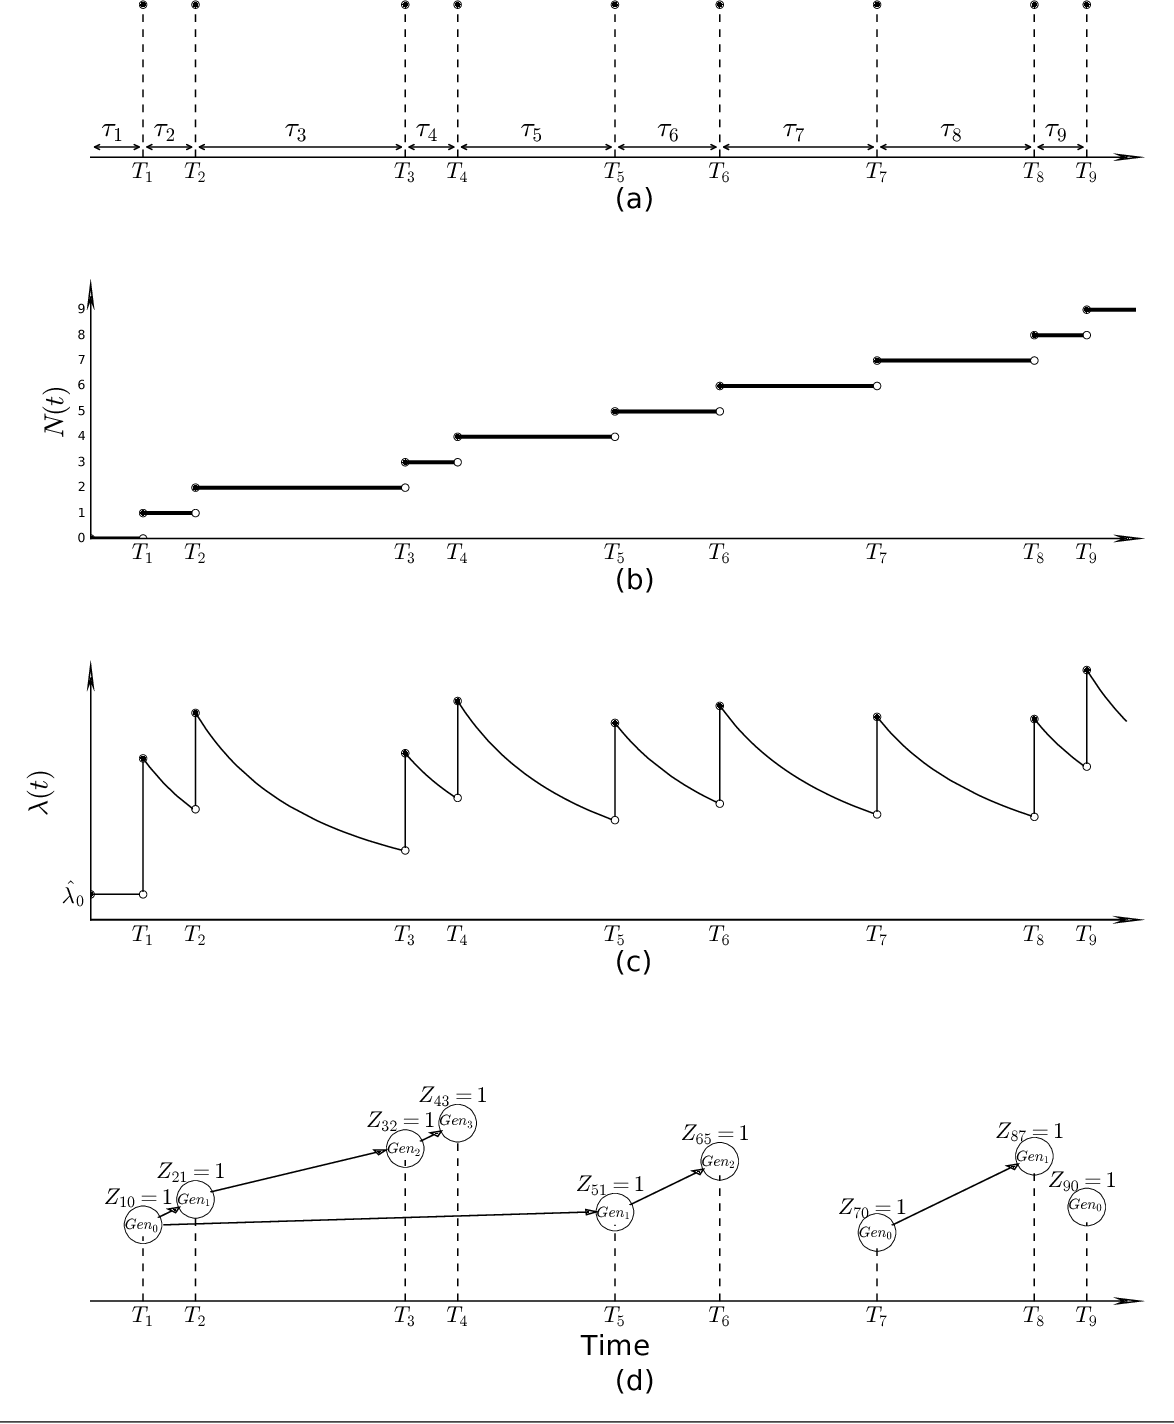
\includegraphics[width=.4\textwidth, trim=0 450 0 0, clip=]{\figcp/Bon24-Hawkes-Fig3}
      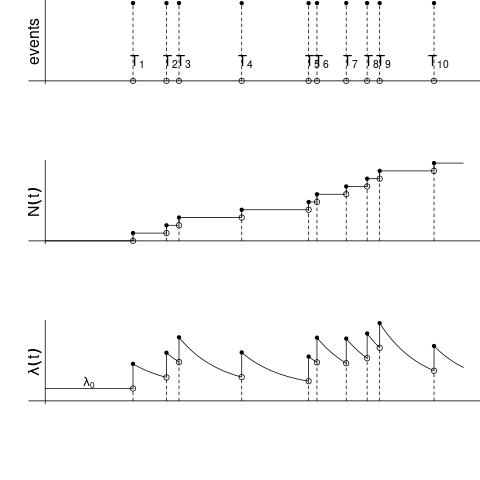
\includegraphics[width=.45\textwidth, trim=0 0 0 0, clip=]{\figcp/FigHawkes-intensity}
    \end{tabular}
    & 
%     \hspace{-.05\textwidth}
    \begin{tabular}{p{.55\textwidth}}
      \begin{itemize}
        \setlength{\itemsep}{.75\baselineskip}
        \item Exponential kernel function \emphase{$h(t)= a e^{-b t}$}
        \item \emphase{$a \geq 0$} to ensure that $\lambda$ is non negative 
        \item \emphase{$a/b <1$} to ensure stationarity
        \item Applications: sismology, epidemiology, vulcanology, neurosciences, ecology, ...
        \goto{sec:Hawkes}
      \end{itemize}
      ~ \\ ~ \\~ \\
    \end{tabular}
  \end{tabular}  

}

%====================================================================
\frame{\frametitle{Simulations: estimation} \label{back:HawkesFit}

  $$
  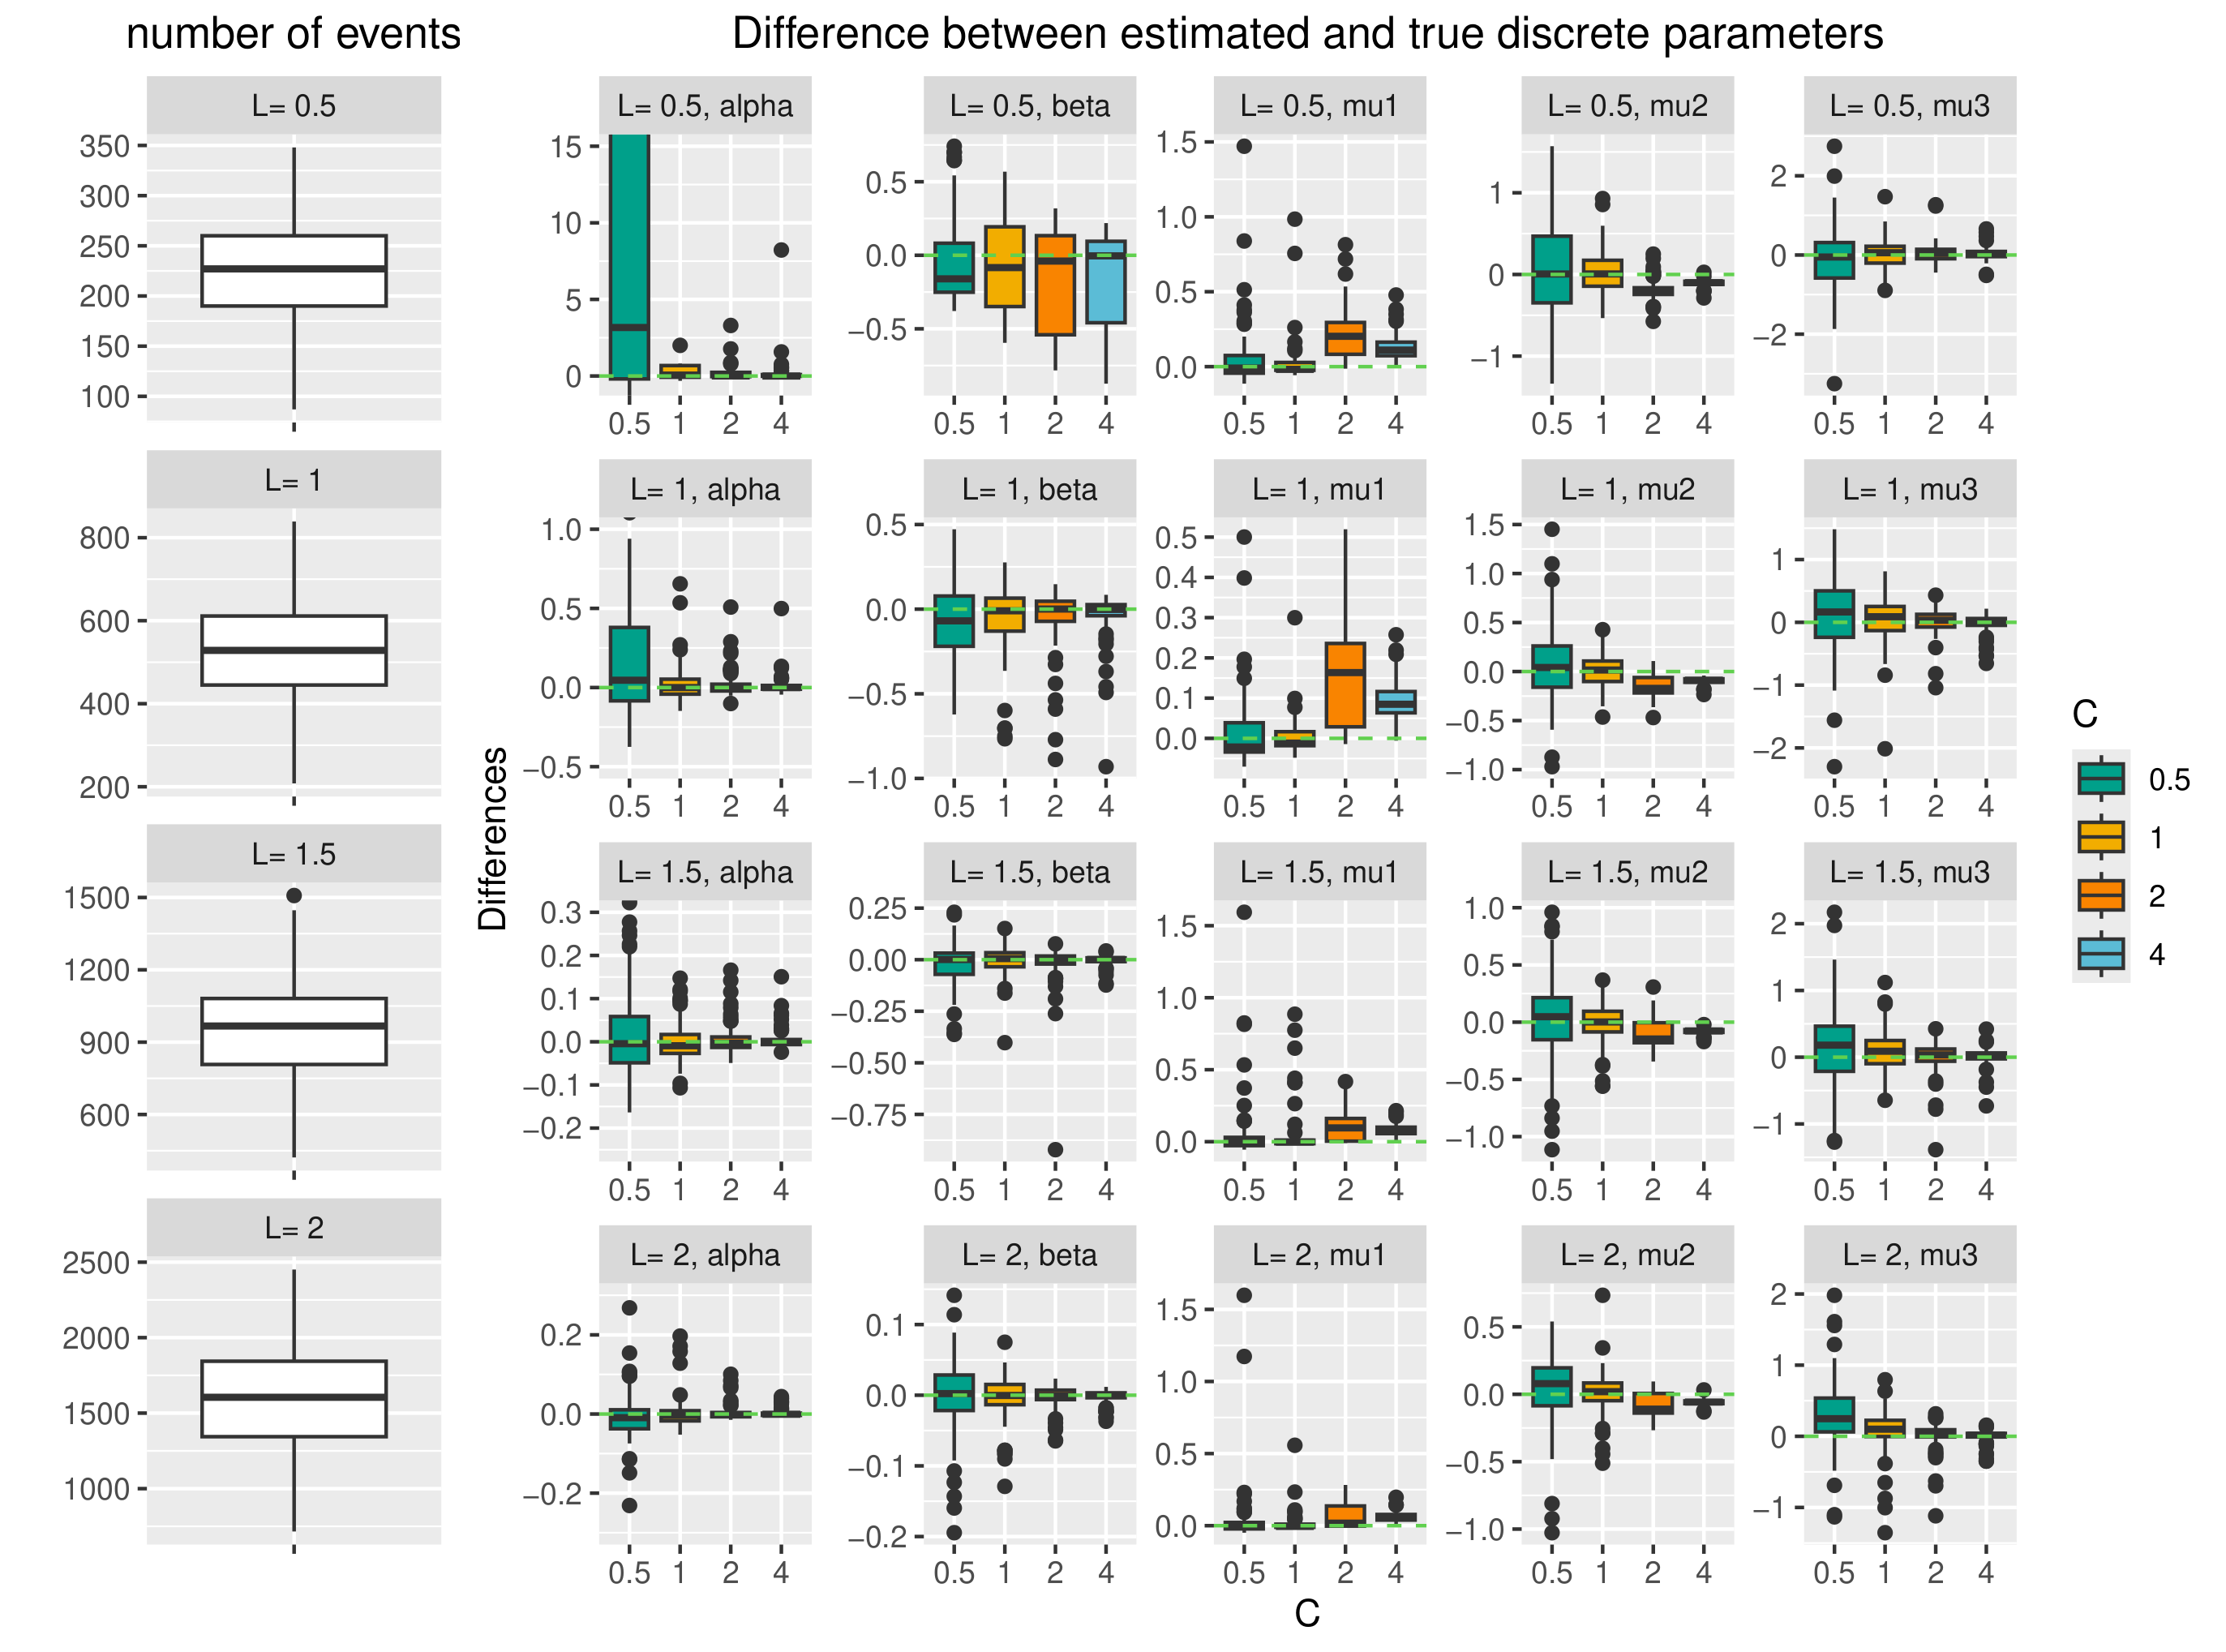
\includegraphics[width=0.75\textwidth]{\figcp/BoR25-ArXiv-disc_parm_scale_ggplot_V8_Q3}
  $$
  \goto{sec:HawkesSimuls}
}

%====================================================================
\frame{\frametitle{Simulations: model selection} \label{back:HawkesAIC}

  $$
  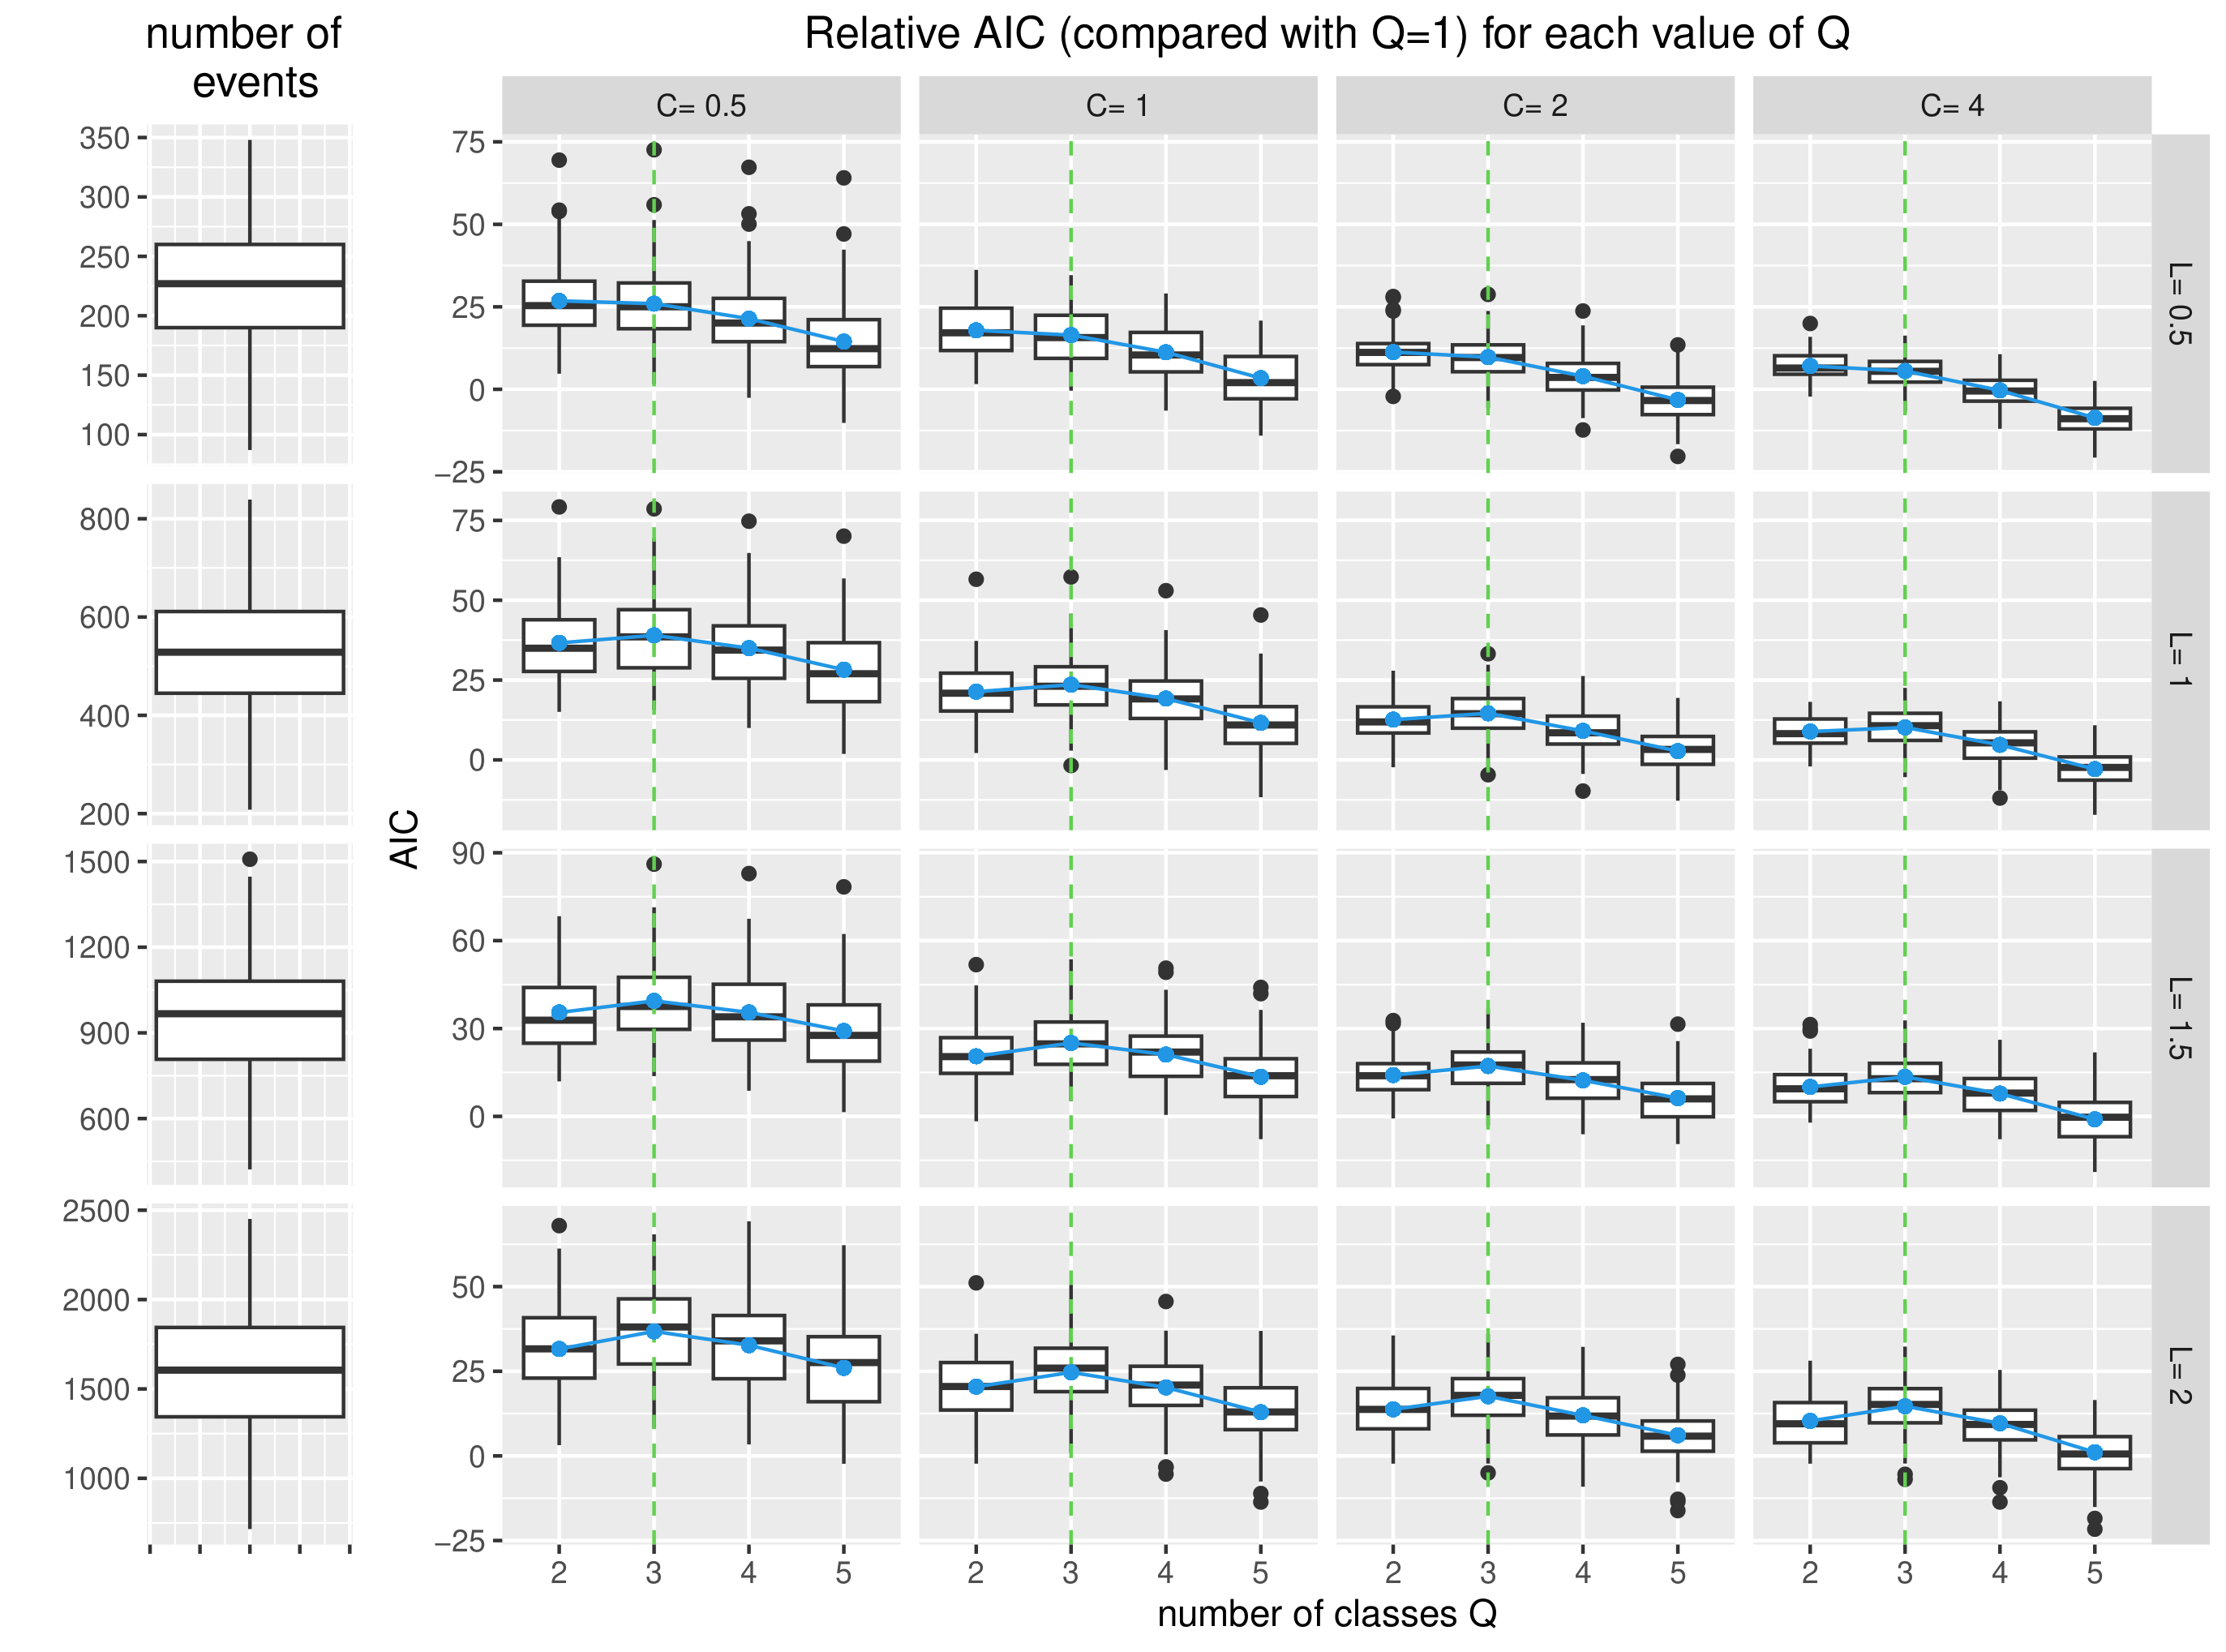
\includegraphics[width=0.75\textwidth]{\figcp/BoR25-ArXiv-aic_ggplot_V8_Q3}
  $$
  \goto{sec:HawkesSimuls}

}

%====================================================================
\frame{\frametitle{Simulations: model selection} \label{back:HawkesClassif}

  $$
  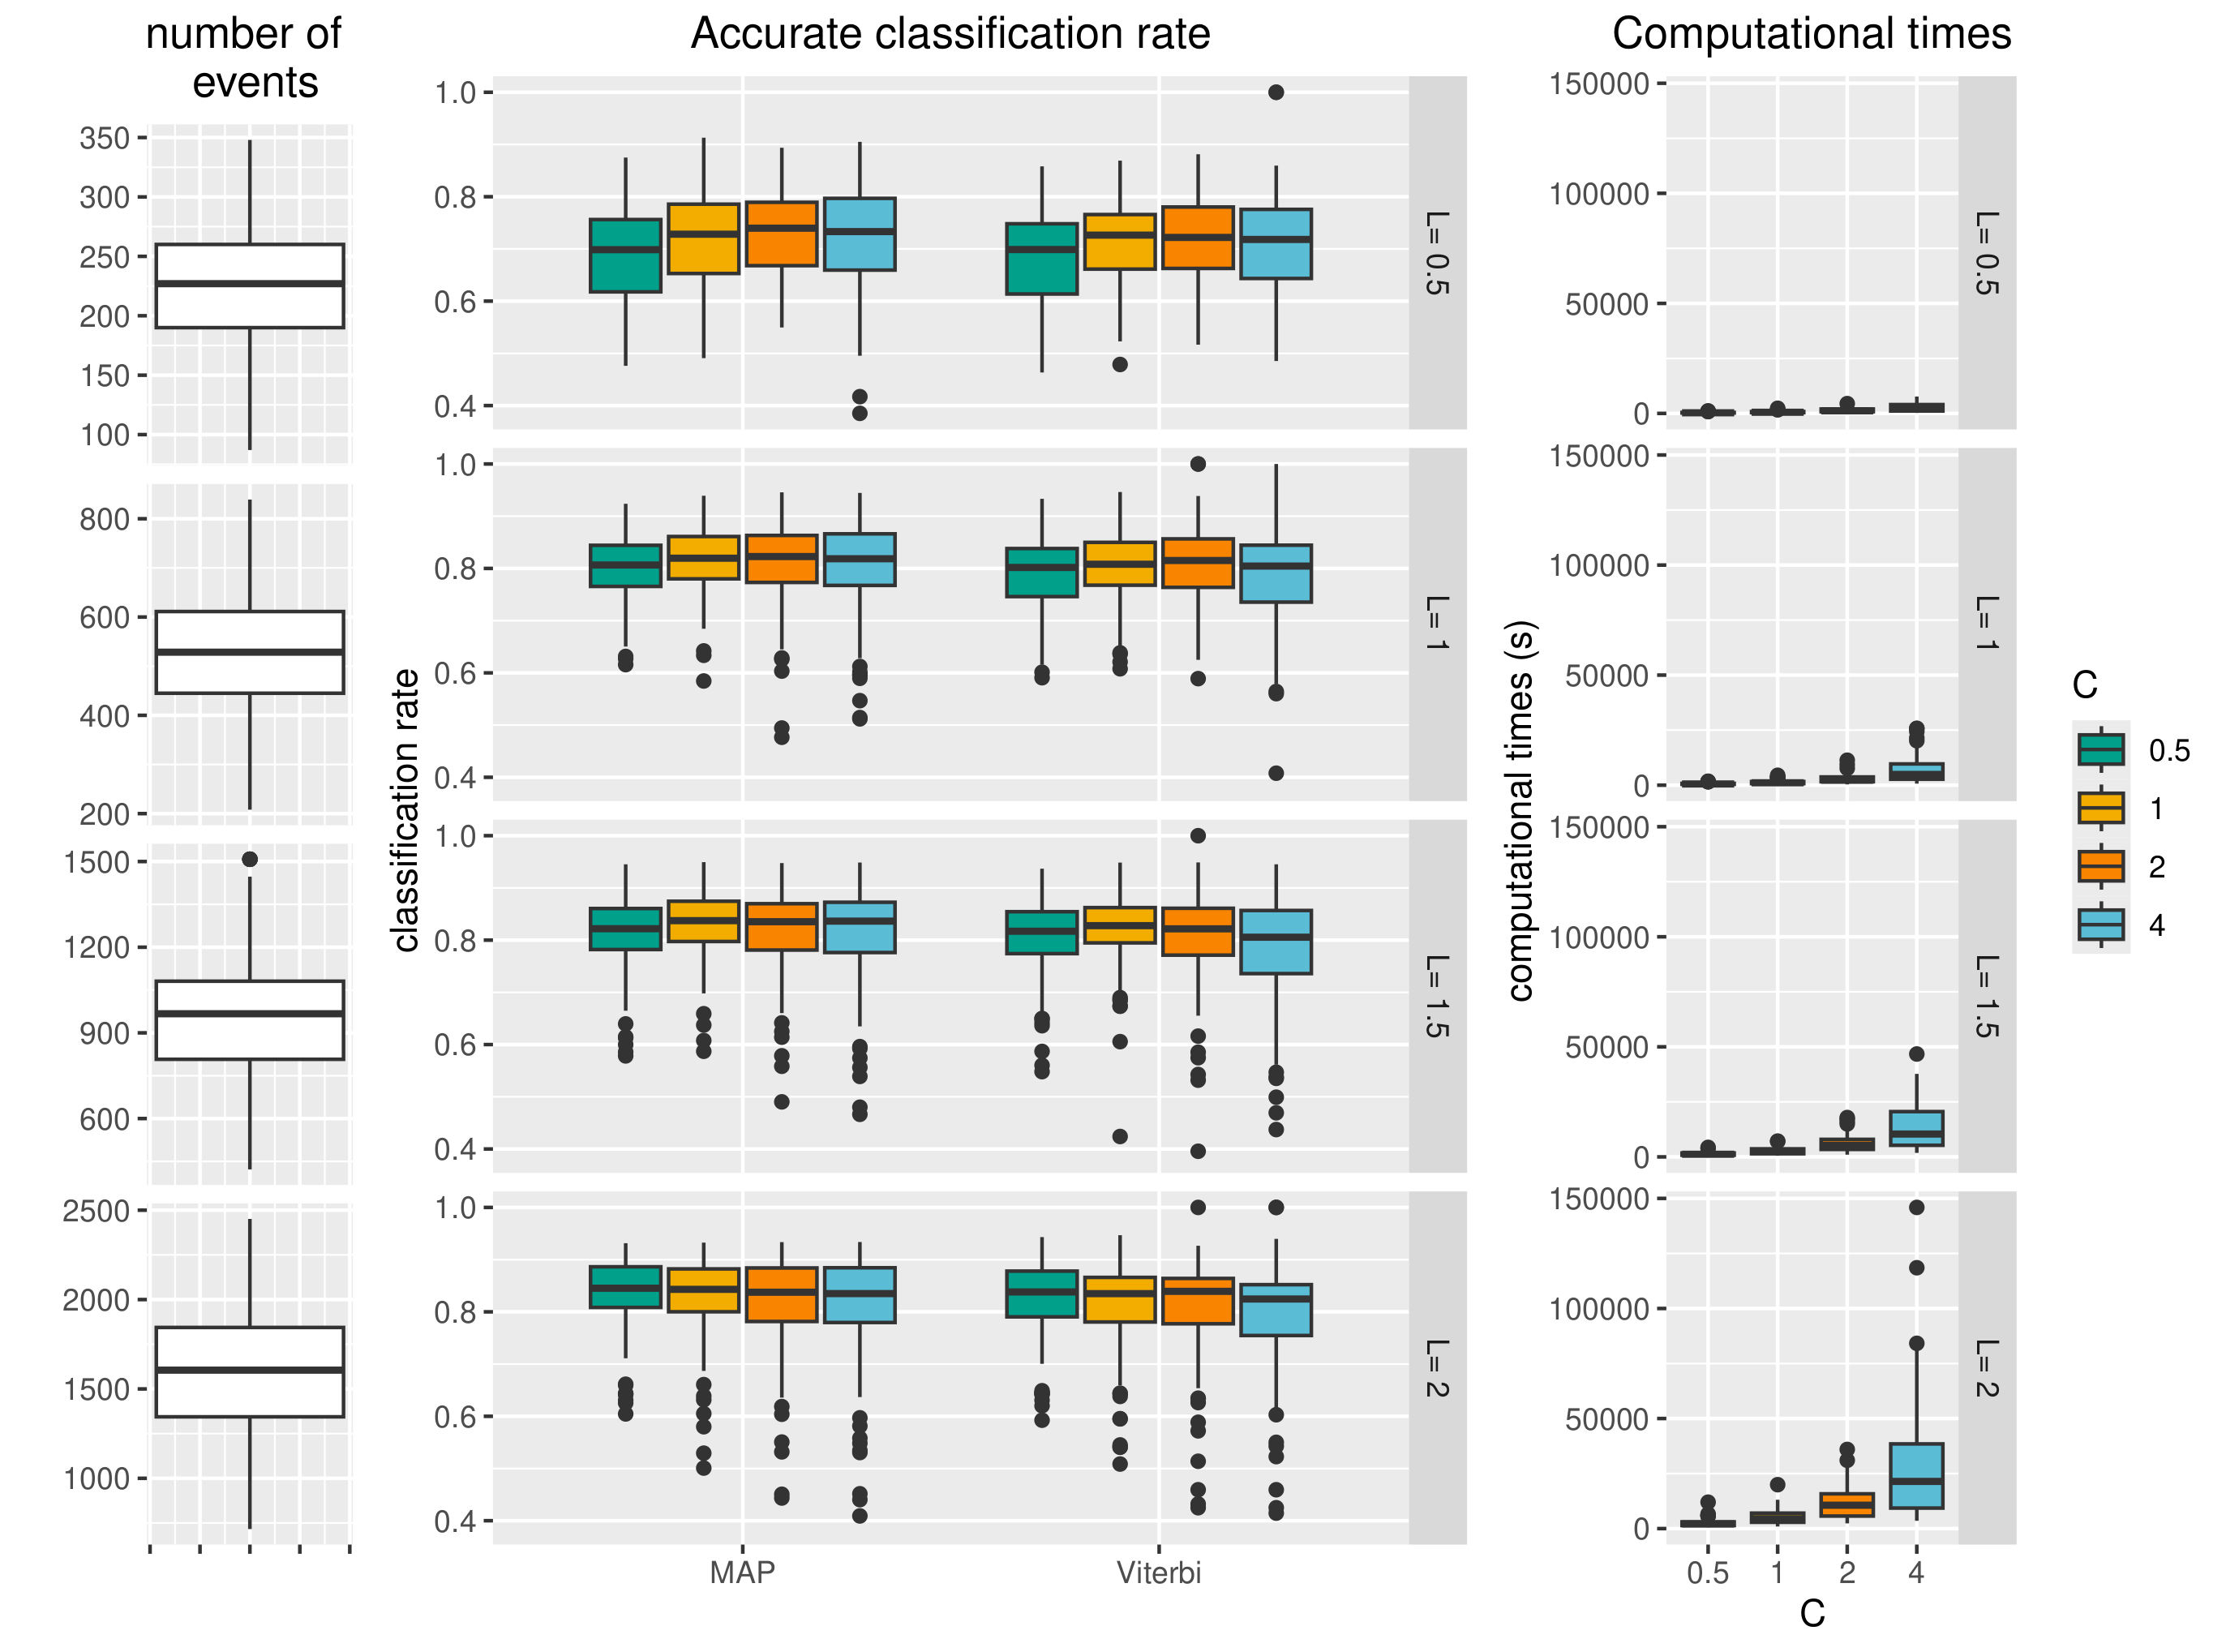
\includegraphics[width=0.75\textwidth]{\figcp/BoR25-ArXiv-classif_cpu_ggplot_V8_Q3}
  $$
  \goto{sec:HawkesSimuls}

}


%====================================================================
\section*{Poisson log-normal model}
%====================================================================
\frame{\frametitle{Barents sea fish abundances: Estimates}

  \paragraph{Reduced data set.} $p = 7$ most abundant species

  \bigskip \bigskip 
  \paragraph{Comparison of the estimates.}
  \newcommand{\nIterEx}{10000} \newcommand{\lagEx}{50} \newcommand{\nISex}{200}
  \newcommand{\exampleParms}{-nIter\nIterEx-lag\lagEx-nIS\nISex}
  \begin{tabular}{ccc}
      $\widehat{B}$ & $\widehat{\Sigma}$ & $\widehat{\Var}(\widehat{B})$  \\
    \includegraphics[width=.3\textwidth, trim=15 40 25 50, clip=]{\figStR/BarentsLarge\exampleParms-compBeta-em-all} &
    \includegraphics[width=.3\textwidth, trim=15 40 25 50, clip=]{\figStR/BarentsLarge\exampleParms-compSigma-em-all} &
    \includegraphics[width=.3\textwidth, trim=15 40 25 50, clip=]{\figStR/BarentsLarge\exampleParms-compVarBeta-em-all}
  \end{tabular}

  }
  
%====================================================================
\frame{\frametitle{Barents sea fish abundances: Model selection}

  \paragraph{BIC for composite likelihood.} \refer{GaS10}
  $$
  BIC = \cl_{\theta}(Y) - \frac{\log(n)}2 \text{dim}(\theta) 
  \qquad \qquad 
  \text{with} \quad
  \text{dim}(\theta) = \tr[J(\theta) H(\theta)^{-1}].
  $$
  
  \bigskip 
  \paragraph{Model selection.} 4 covariates $\to$ 16 possible models 
  \newcommand{\nIterEx}{10000} \newcommand{\lagEx}{50} \newcommand{\nISex}{200}
  \newcommand{\exampleParms}{-nIter\nIterEx-lag\lagEx-nIS\nISex}
  \newcommand{\nIterSel}{\nIterEx} \newcommand{\lagSel}{20} \newcommand{\nISsel}{\nISex}
  \newcommand{\selectParms}{-nIS\nISsel-nIter\nIterSel-lag\lagSel}
  $$
  \begin{tabular}{ccc}
    $\cl_{\widehat{\theta}_k}$ & $\text{dim}(\widehat{\theta}_k)$ & $BIC(k)$ \\
    \includegraphics[width=.25\textwidth, trim=10 10 25 50, clip=]{\figStR/Barents\selectParms-models-cl} & 
    \includegraphics[width=.25\textwidth, trim=10 10 25 50, clip=]{\figStR/Barents\selectParms-models-penbic} & 
    \includegraphics[width=.25\textwidth, trim=10 10 25 50, clip=]{\figStR/Barents\selectParms-models-bic}     
  \end{tabular}
  $$
  CL(5) vs CL(7): same for $d=1, 2, 3$ and 5 (best) \\
  \medskip 
  Differ only for $d=4$: \\
  CL5 = Latitude + Depth + Temperature, CL7 = Latitude + Depth + Longitude

}


\backupend 

%====================================================================
%====================================================================
\end{document}
%====================================================================
%====================================================================
  
  \begin{tabular}{cc}
    \hspace{-.04\textwidth}
    \begin{tabular}{p{.5\textwidth}}
    \end{tabular}
    & 
    \hspace{-.02\textwidth}
    \begin{tabular}{p{.5\textwidth}}
    \end{tabular}
  \end{tabular}
